% Options for packages loaded elsewhere
\PassOptionsToPackage{unicode}{hyperref}
\PassOptionsToPackage{hyphens}{url}
%
\documentclass[
]{article}
\usepackage{amsmath,amssymb}
\usepackage{lmodern}
\usepackage{iftex}
\ifPDFTeX
  \usepackage[T1]{fontenc}
  \usepackage[utf8]{inputenc}
  \usepackage{textcomp} % provide euro and other symbols
\else % if luatex or xetex
  \usepackage{unicode-math}
  \defaultfontfeatures{Scale=MatchLowercase}
  \defaultfontfeatures[\rmfamily]{Ligatures=TeX,Scale=1}
\fi
% Use upquote if available, for straight quotes in verbatim environments
\IfFileExists{upquote.sty}{\usepackage{upquote}}{}
\IfFileExists{microtype.sty}{% use microtype if available
  \usepackage[]{microtype}
  \UseMicrotypeSet[protrusion]{basicmath} % disable protrusion for tt fonts
}{}
\makeatletter
\@ifundefined{KOMAClassName}{% if non-KOMA class
  \IfFileExists{parskip.sty}{%
    \usepackage{parskip}
  }{% else
    \setlength{\parindent}{0pt}
    \setlength{\parskip}{6pt plus 2pt minus 1pt}}
}{% if KOMA class
  \KOMAoptions{parskip=half}}
\makeatother
\usepackage{xcolor}
\IfFileExists{xurl.sty}{\usepackage{xurl}}{} % add URL line breaks if available
\IfFileExists{bookmark.sty}{\usepackage{bookmark}}{\usepackage{hyperref}}
\hypersetup{
  hidelinks,
  pdfcreator={LaTeX via pandoc}}
\urlstyle{same} % disable monospaced font for URLs
\usepackage[margin=1in]{geometry}
\usepackage{color}
\usepackage{fancyvrb}
\newcommand{\VerbBar}{|}
\newcommand{\VERB}{\Verb[commandchars=\\\{\}]}
\DefineVerbatimEnvironment{Highlighting}{Verbatim}{commandchars=\\\{\}}
% Add ',fontsize=\small' for more characters per line
\usepackage{framed}
\definecolor{shadecolor}{RGB}{248,248,248}
\newenvironment{Shaded}{\begin{snugshade}}{\end{snugshade}}
\newcommand{\AlertTok}[1]{\textcolor[rgb]{0.94,0.16,0.16}{#1}}
\newcommand{\AnnotationTok}[1]{\textcolor[rgb]{0.56,0.35,0.01}{\textbf{\textit{#1}}}}
\newcommand{\AttributeTok}[1]{\textcolor[rgb]{0.77,0.63,0.00}{#1}}
\newcommand{\BaseNTok}[1]{\textcolor[rgb]{0.00,0.00,0.81}{#1}}
\newcommand{\BuiltInTok}[1]{#1}
\newcommand{\CharTok}[1]{\textcolor[rgb]{0.31,0.60,0.02}{#1}}
\newcommand{\CommentTok}[1]{\textcolor[rgb]{0.56,0.35,0.01}{\textit{#1}}}
\newcommand{\CommentVarTok}[1]{\textcolor[rgb]{0.56,0.35,0.01}{\textbf{\textit{#1}}}}
\newcommand{\ConstantTok}[1]{\textcolor[rgb]{0.00,0.00,0.00}{#1}}
\newcommand{\ControlFlowTok}[1]{\textcolor[rgb]{0.13,0.29,0.53}{\textbf{#1}}}
\newcommand{\DataTypeTok}[1]{\textcolor[rgb]{0.13,0.29,0.53}{#1}}
\newcommand{\DecValTok}[1]{\textcolor[rgb]{0.00,0.00,0.81}{#1}}
\newcommand{\DocumentationTok}[1]{\textcolor[rgb]{0.56,0.35,0.01}{\textbf{\textit{#1}}}}
\newcommand{\ErrorTok}[1]{\textcolor[rgb]{0.64,0.00,0.00}{\textbf{#1}}}
\newcommand{\ExtensionTok}[1]{#1}
\newcommand{\FloatTok}[1]{\textcolor[rgb]{0.00,0.00,0.81}{#1}}
\newcommand{\FunctionTok}[1]{\textcolor[rgb]{0.00,0.00,0.00}{#1}}
\newcommand{\ImportTok}[1]{#1}
\newcommand{\InformationTok}[1]{\textcolor[rgb]{0.56,0.35,0.01}{\textbf{\textit{#1}}}}
\newcommand{\KeywordTok}[1]{\textcolor[rgb]{0.13,0.29,0.53}{\textbf{#1}}}
\newcommand{\NormalTok}[1]{#1}
\newcommand{\OperatorTok}[1]{\textcolor[rgb]{0.81,0.36,0.00}{\textbf{#1}}}
\newcommand{\OtherTok}[1]{\textcolor[rgb]{0.56,0.35,0.01}{#1}}
\newcommand{\PreprocessorTok}[1]{\textcolor[rgb]{0.56,0.35,0.01}{\textit{#1}}}
\newcommand{\RegionMarkerTok}[1]{#1}
\newcommand{\SpecialCharTok}[1]{\textcolor[rgb]{0.00,0.00,0.00}{#1}}
\newcommand{\SpecialStringTok}[1]{\textcolor[rgb]{0.31,0.60,0.02}{#1}}
\newcommand{\StringTok}[1]{\textcolor[rgb]{0.31,0.60,0.02}{#1}}
\newcommand{\VariableTok}[1]{\textcolor[rgb]{0.00,0.00,0.00}{#1}}
\newcommand{\VerbatimStringTok}[1]{\textcolor[rgb]{0.31,0.60,0.02}{#1}}
\newcommand{\WarningTok}[1]{\textcolor[rgb]{0.56,0.35,0.01}{\textbf{\textit{#1}}}}
\usepackage{graphicx}
\makeatletter
\def\maxwidth{\ifdim\Gin@nat@width>\linewidth\linewidth\else\Gin@nat@width\fi}
\def\maxheight{\ifdim\Gin@nat@height>\textheight\textheight\else\Gin@nat@height\fi}
\makeatother
% Scale images if necessary, so that they will not overflow the page
% margins by default, and it is still possible to overwrite the defaults
% using explicit options in \includegraphics[width, height, ...]{}
\setkeys{Gin}{width=\maxwidth,height=\maxheight,keepaspectratio}
% Set default figure placement to htbp
\makeatletter
\def\fps@figure{htbp}
\makeatother
\setlength{\emergencystretch}{3em} % prevent overfull lines
\providecommand{\tightlist}{%
  \setlength{\itemsep}{0pt}\setlength{\parskip}{0pt}}
\setcounter{secnumdepth}{-\maxdimen} % remove section numbering
\usepackage{subfig}
\ifLuaTeX
  \usepackage{selnolig}  % disable illegal ligatures
\fi

\author{}
\date{\vspace{-2.5em}}

\begin{document}

\begin{verbatim}
## Warning: le package 'randtoolbox' a été compilé avec la version R 4.2.2
\end{verbatim}

\begin{verbatim}
## Warning: le package 'rngWELL' a été compilé avec la version R 4.2.2
\end{verbatim}

\thispagestyle{empty}
\begin{center}
  \vspace*{\stretch{1}}
  {\scshape \huge Génération de nombres aléatoires et probabilités\\}
  \vspace{2em}
  Billy VILLEROY Hélène DOS SANTOS Seynabou SARR\\
  \vspace*{\stretch{2}}
  3IF 2022-2023
\end{center}
\clearpage
\thispagestyle{empty}
\clearpage
\thispagestyle{empty}
\tableofcontents
\clearpage
\part*{Partie I : Générateurs pseudo-aléatoires}
\addcontentsline{toc}{part}{Générateurs pseudo-aléatoires}
\section*{1. Mise en place et études graphiques}
\addcontentsline{toc}{subsection}{Mise en place et études graphiques}

\subsection*{A. Exemples}

\paragraph{}

Dans un premier temps, nous avons généré des nombres pseudo-aléatoires à
l'aide de l'ensemble des générateurs dont vous retrouverez
l'implémentation dans les
annexes\footnote{Voir p. \pageref{part:annexes}}. Voici les résultats
obtenus :

\begin{itemize}
  \item L'histogramme représente la fréquence d'apparition des nombres sur l'intervalle en ordonnée.
  \item Le graphique représente chaque nombre en fonction de celui qui lui précède, il permet d'évaluer l'étendue, entre les valeurs, générée par l'algorithme.
\end{itemize}
\vspace*{\stretch{1}}
\begin{figure}

{\centering \subfloat[Fréquence d'apparition des nombres générés\label{fig:unnamed-chunk-2-1}]{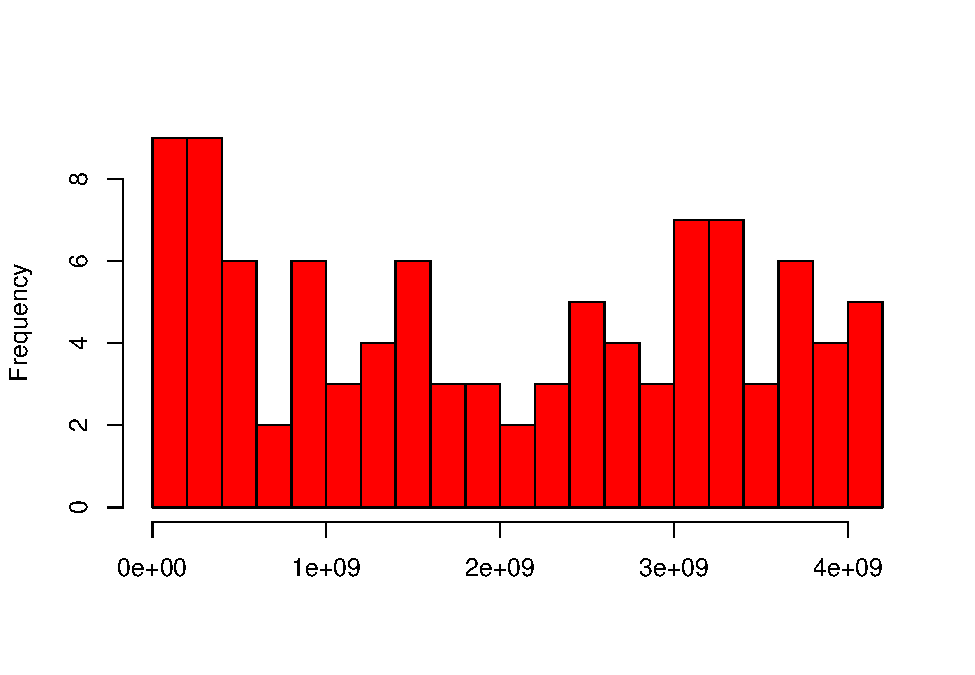
\includegraphics[width=0.5\linewidth]{CRTP_PROBA_files/figure-latex/unnamed-chunk-2-1} }\subfloat[Sucesseurs en fonction des prédecesseurs\label{fig:unnamed-chunk-2-2}]{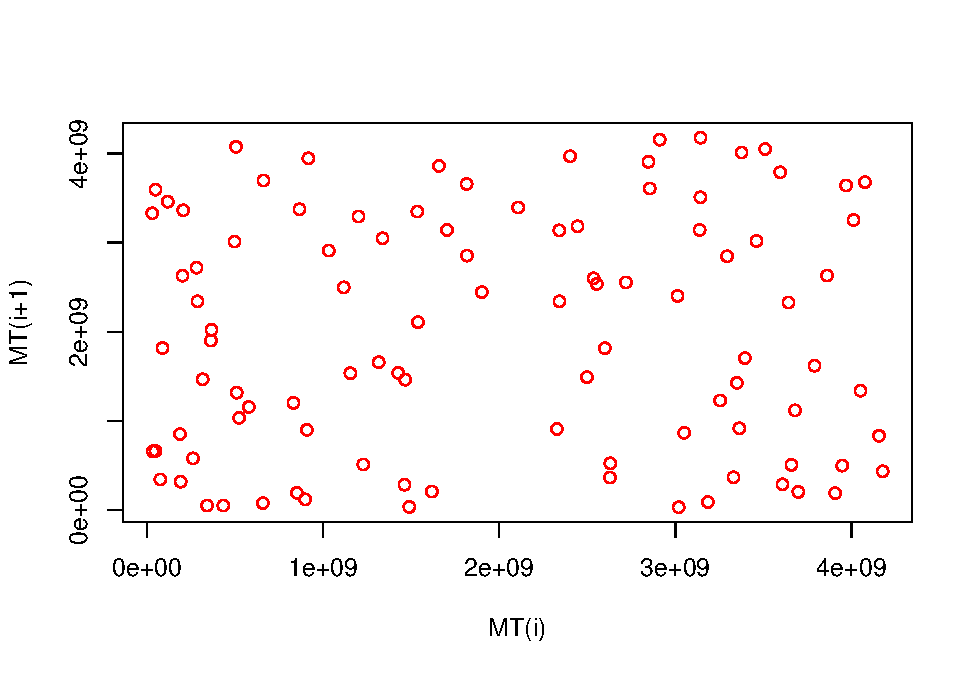
\includegraphics[width=0.5\linewidth]{CRTP_PROBA_files/figure-latex/unnamed-chunk-2-2} }

}

\caption{Générateur de Mersenne Twister (Graine : 1502, 100 générations)}\label{fig:unnamed-chunk-2}
\end{figure}
\vspace*{\stretch{1}}
\begin{figure}

{\centering \subfloat[Fréquence d'apparition des nombres générés\label{fig:unnamed-chunk-3-1}]{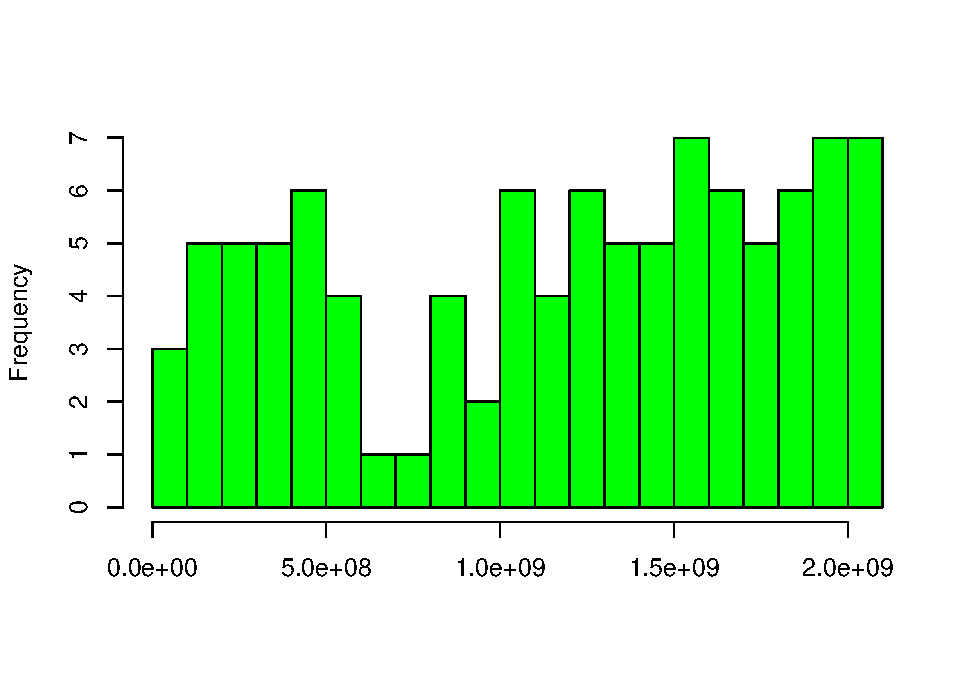
\includegraphics[width=0.5\linewidth]{CRTP_PROBA_files/figure-latex/unnamed-chunk-3-1} }\subfloat[Sucesseurs en fonction des prédecesseurs\label{fig:unnamed-chunk-3-2}]{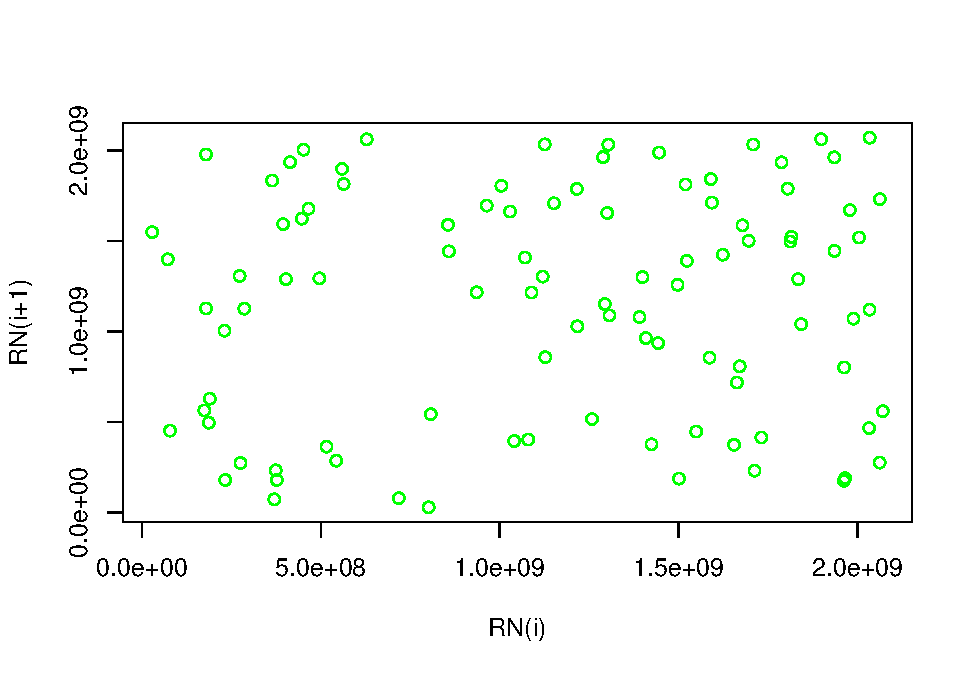
\includegraphics[width=0.5\linewidth]{CRTP_PROBA_files/figure-latex/unnamed-chunk-3-2} }

}

\caption{Générateur RANDU (Graine : 5645, 100 générations)}\label{fig:unnamed-chunk-3}
\end{figure}

\begin{figure}

{\centering \subfloat[Fréquence d'apparition des nombres générés\label{fig:unnamed-chunk-4-1}]{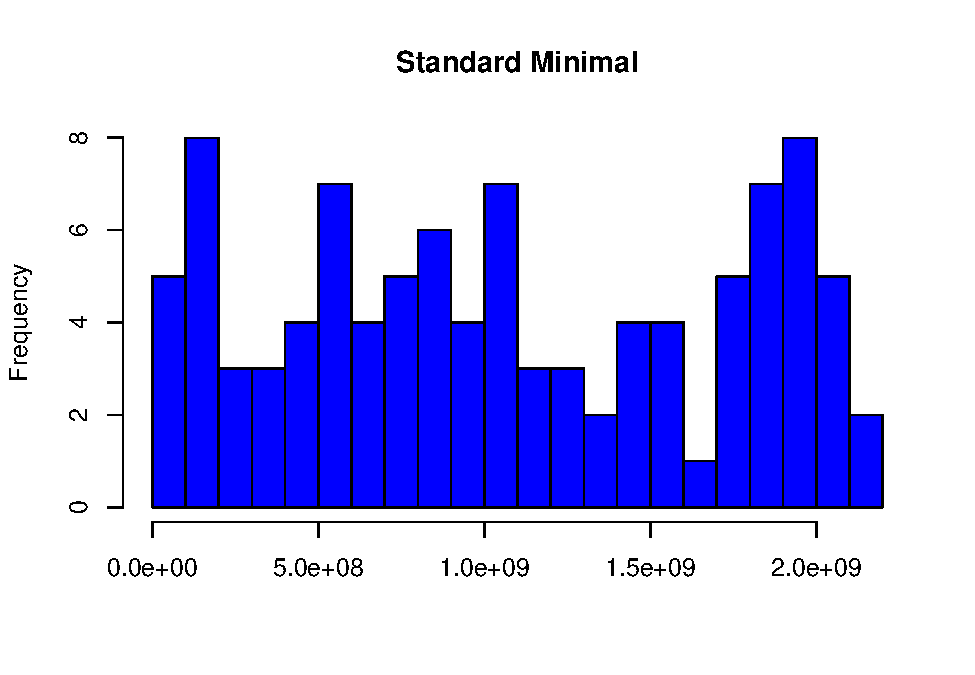
\includegraphics[width=0.5\linewidth]{CRTP_PROBA_files/figure-latex/unnamed-chunk-4-1} }\subfloat[Sucesseurs en fonction des prédecesseurs\label{fig:unnamed-chunk-4-2}]{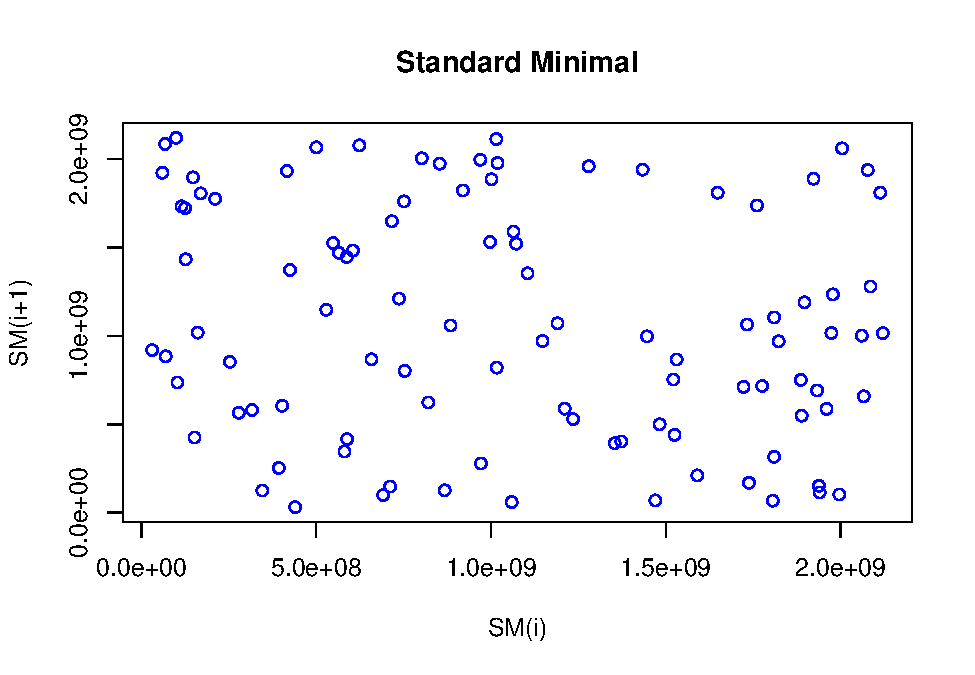
\includegraphics[width=0.5\linewidth]{CRTP_PROBA_files/figure-latex/unnamed-chunk-4-2} }

}

\caption{Générateur Standard Minimal (Graine : 9575, 100 générations)}\label{fig:unnamed-chunk-4}
\end{figure}

\begin{figure}

{\centering \subfloat[Fréquence d'apparition des nombres générés\label{fig:unnamed-chunk-5-1}]{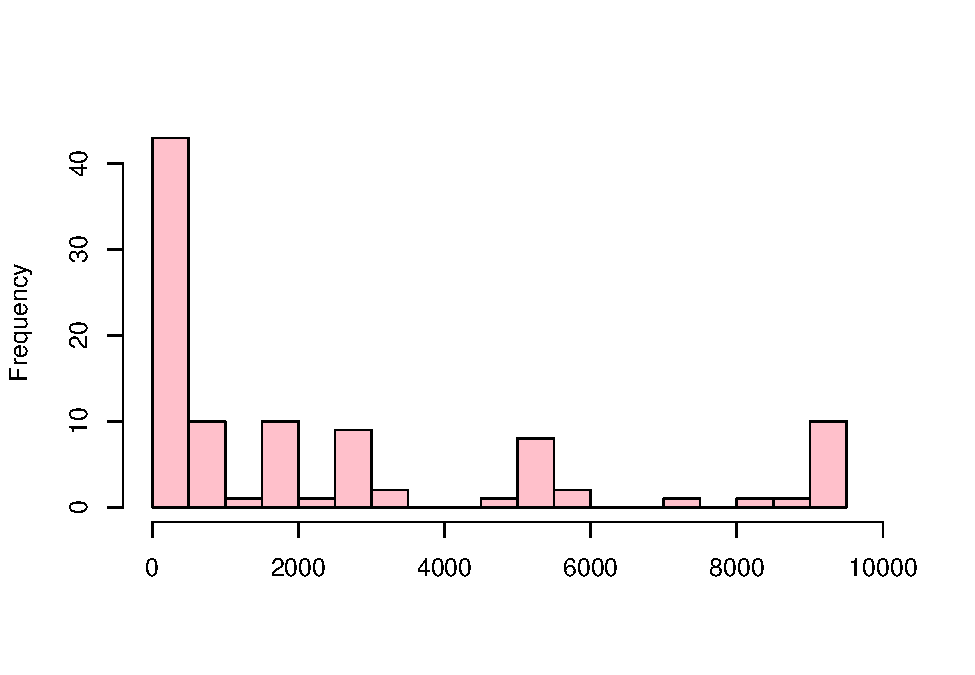
\includegraphics[width=0.5\linewidth]{CRTP_PROBA_files/figure-latex/unnamed-chunk-5-1} }\subfloat[Sucesseurs en fonction des prédecesseurs\label{fig:unnamed-chunk-5-2}]{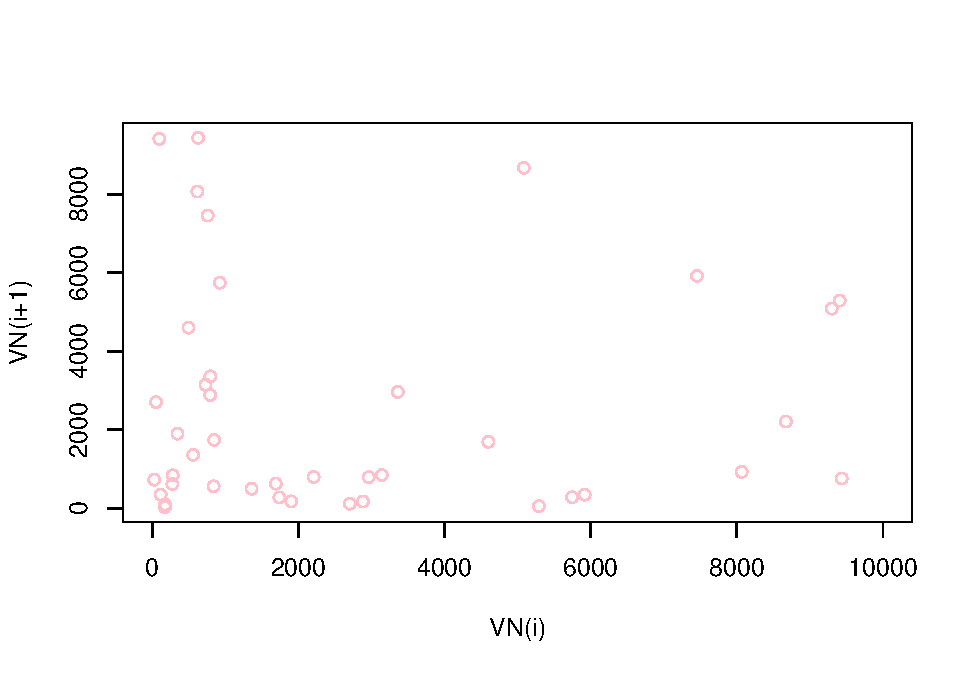
\includegraphics[width=0.5\linewidth]{CRTP_PROBA_files/figure-latex/unnamed-chunk-5-2} }

}

\caption{Générateur de Von Neuman (Graine : 3454, 100 générations)}\label{fig:unnamed-chunk-5}
\end{figure}

\clearpage

\subsection*{B. Vision globale}

\paragraph{}

Pour donner une vision d'ensemble, nous avons généré 100 séquences avec
des
graines\footnote{Vous pouvez les retrouver p. \pageref{part:annexes}}
produites par la fonction \textbf{sample} de R :

\begin{figure}
\subfloat[Mersenne Twister\label{fig:unnamed-chunk-6-1}]{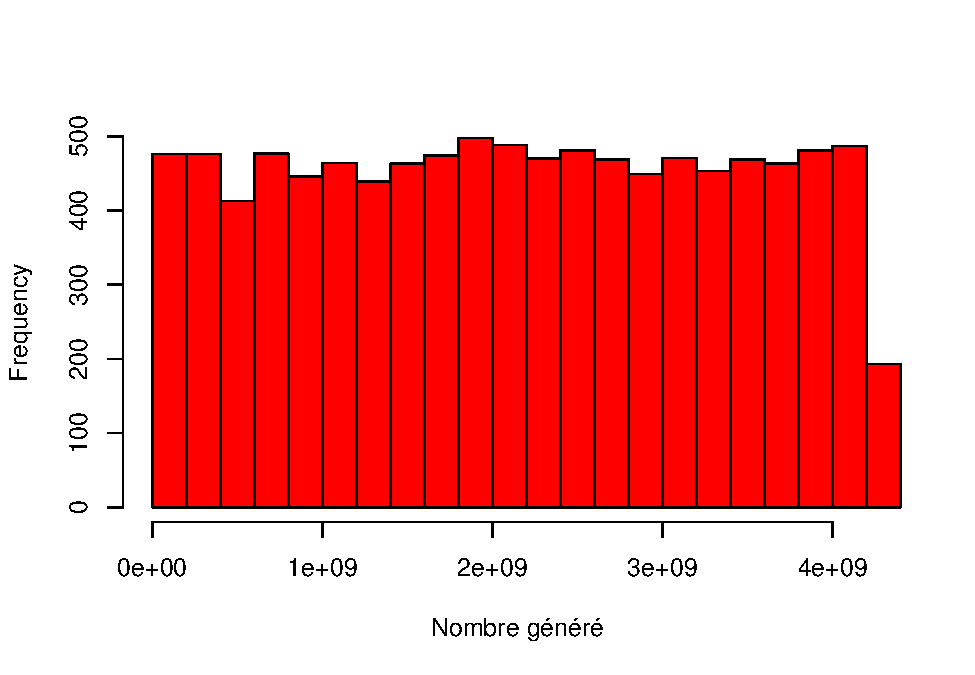
\includegraphics[width=0.5\linewidth]{CRTP_PROBA_files/figure-latex/unnamed-chunk-6-1} }\subfloat[Von Neuman\label{fig:unnamed-chunk-6-2}]{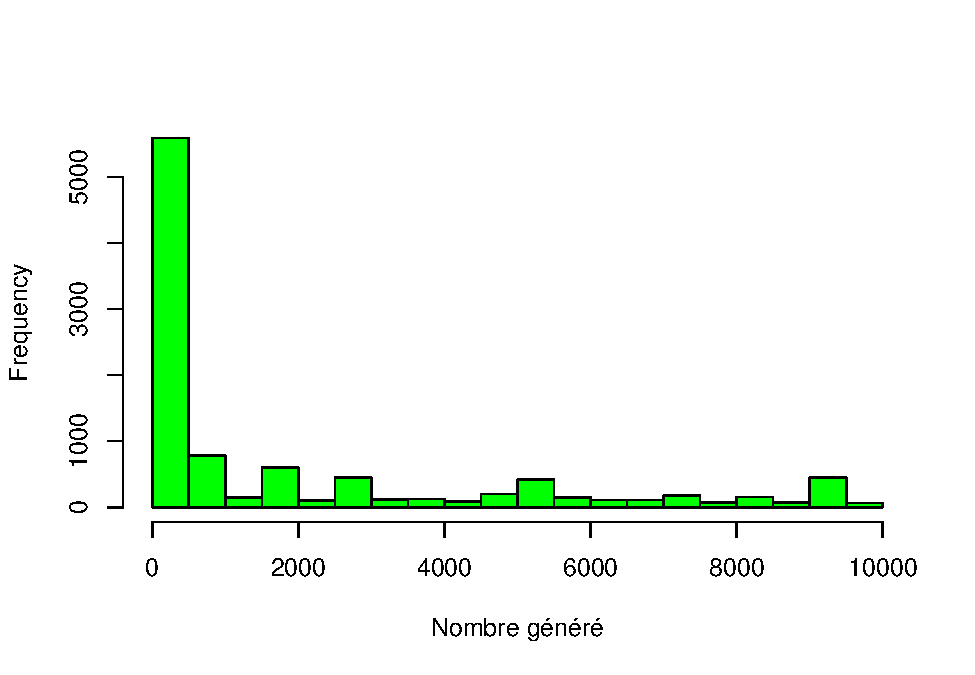
\includegraphics[width=0.5\linewidth]{CRTP_PROBA_files/figure-latex/unnamed-chunk-6-2} }\newline\subfloat[RANDU\label{fig:unnamed-chunk-6-3}]{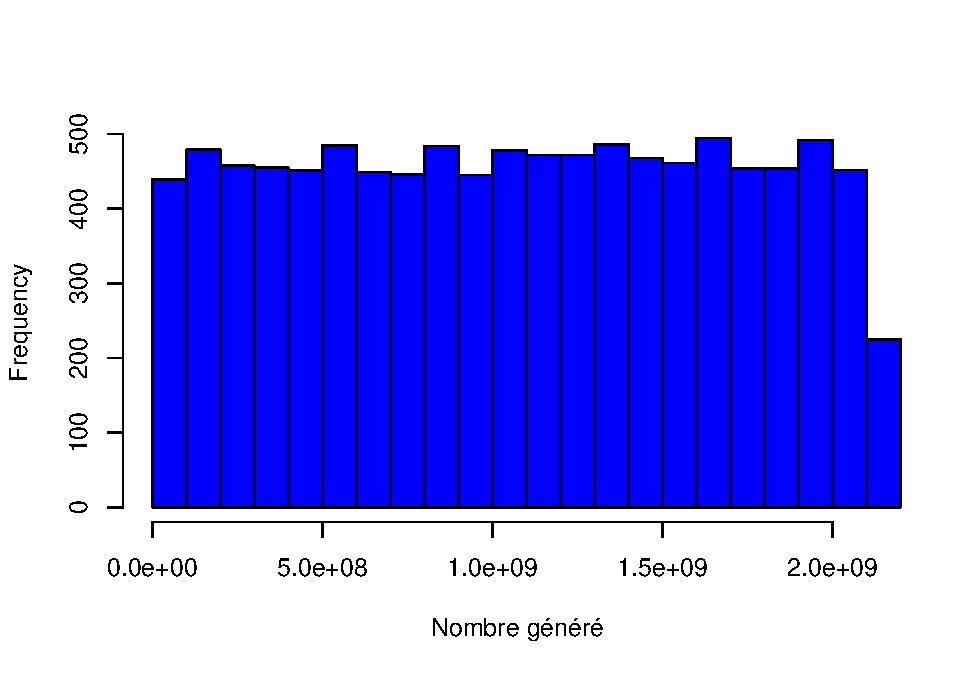
\includegraphics[width=0.5\linewidth]{CRTP_PROBA_files/figure-latex/unnamed-chunk-6-3} }\subfloat[Standard Minimal\label{fig:unnamed-chunk-6-4}]{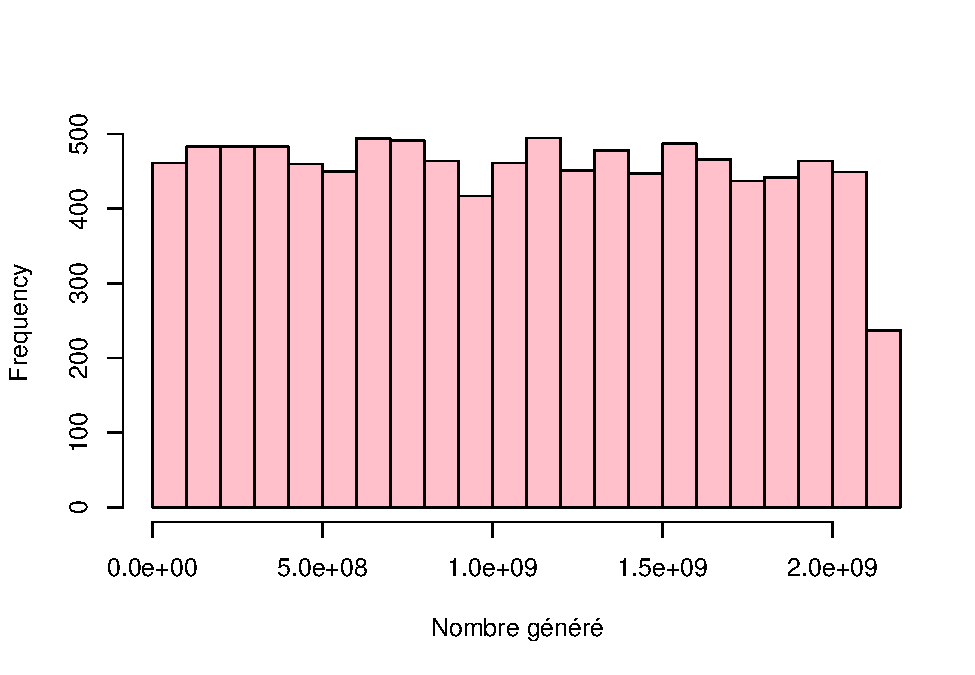
\includegraphics[width=0.5\linewidth]{CRTP_PROBA_files/figure-latex/unnamed-chunk-6-4} }\caption{Etude sur 100 séquences de cardinal 100, Graine aléatoire}\label{fig:unnamed-chunk-6}
\end{figure}

\textbf{Analyse graphique}

\paragraph{}

Dans l'ensemble, les nombres produits sont bien répartis sur les
intervalles considérés à part pour Von Neuman, qui génère une majorité
de nombres inférieurs à 2000. Mais cela n'est qu'une apréciation
visuelle, par la suite nous allons effectuer divers tests sur nos
générateurs afin de déterminer si les nombres et séquences produites
peuvent êtres considérés comme aléatoires.

\clearpage
\section*{2. Etudes probabilistes}
\addcontentsline{toc}{subsection}{Etudes probabilistes}

Les deux premières parties traitent de tests réalisés sur les
bits\footnote{Générés par la fonction \textit{binary}, p. \pageref{subsec:binary}}
des nombres générés.

\subsection*{A. Tests de répartition\footnote{Voir \textit{Frequency} p. \pageref{frequency}}}
\begin{figure}
\subfloat[Mersenne Twister\label{fig:unnamed-chunk-7-1}]{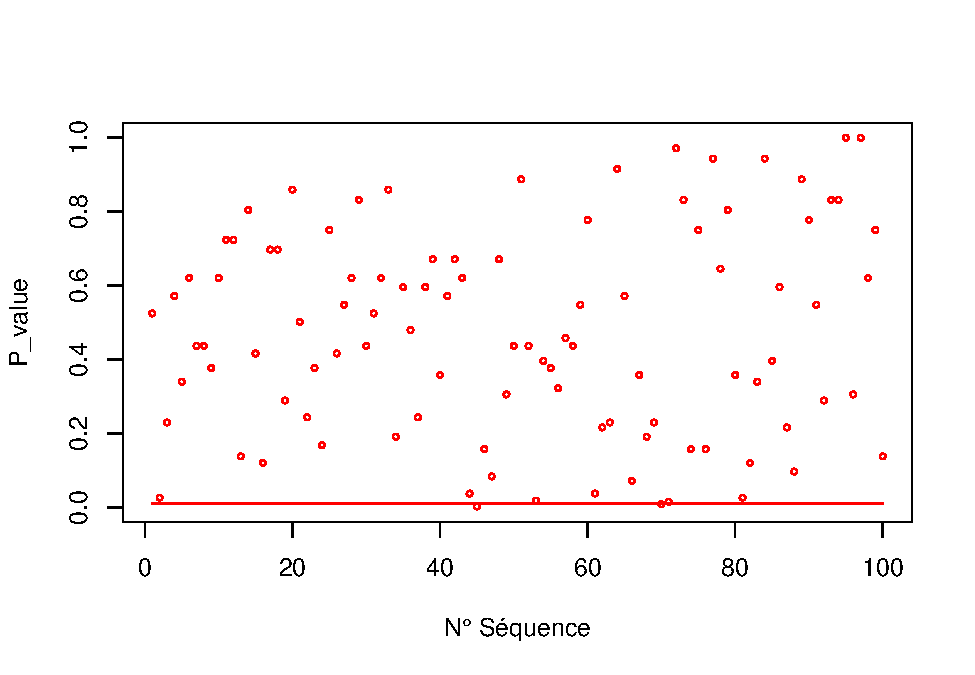
\includegraphics[width=0.5\linewidth]{CRTP_PROBA_files/figure-latex/unnamed-chunk-7-1} }\subfloat[Von Neuman\label{fig:unnamed-chunk-7-2}]{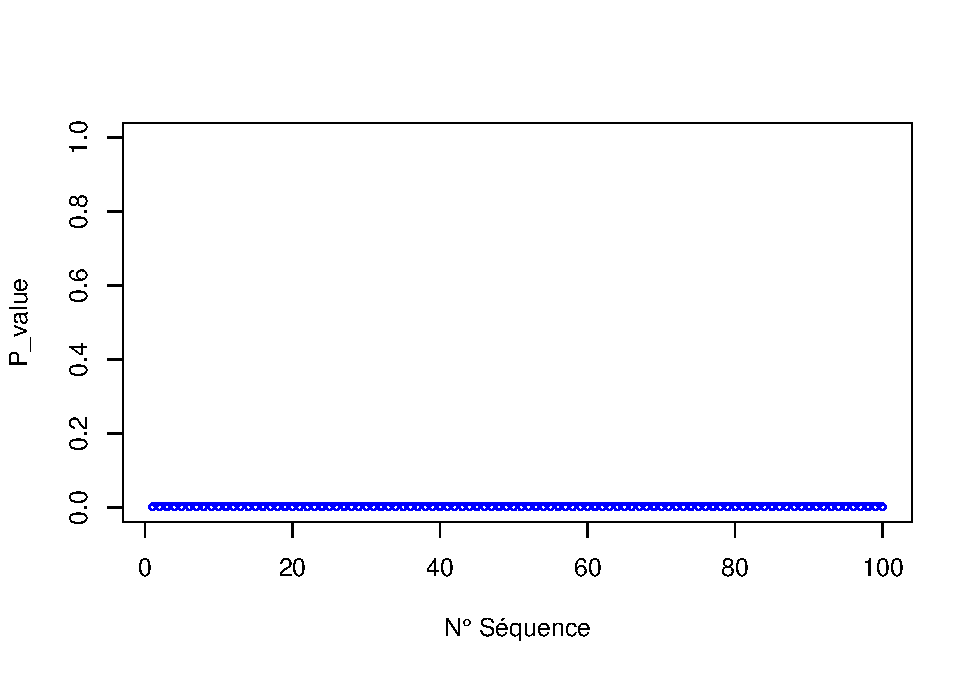
\includegraphics[width=0.5\linewidth]{CRTP_PROBA_files/figure-latex/unnamed-chunk-7-2} }\newline\subfloat[RANDU\label{fig:unnamed-chunk-7-3}]{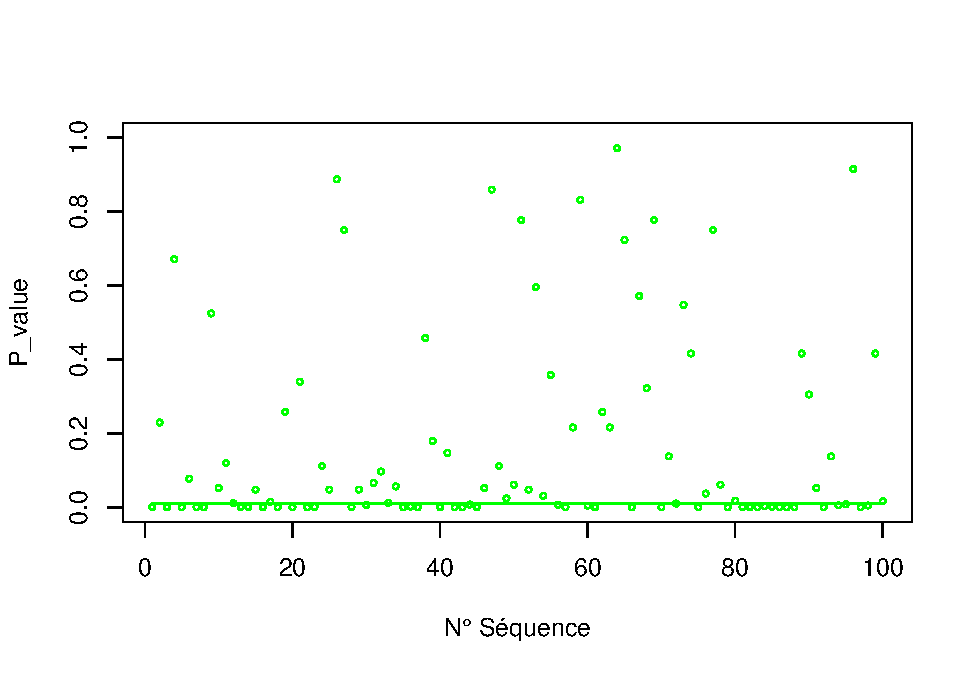
\includegraphics[width=0.5\linewidth]{CRTP_PROBA_files/figure-latex/unnamed-chunk-7-3} }\subfloat[Standard Minimal\label{fig:unnamed-chunk-7-4}]{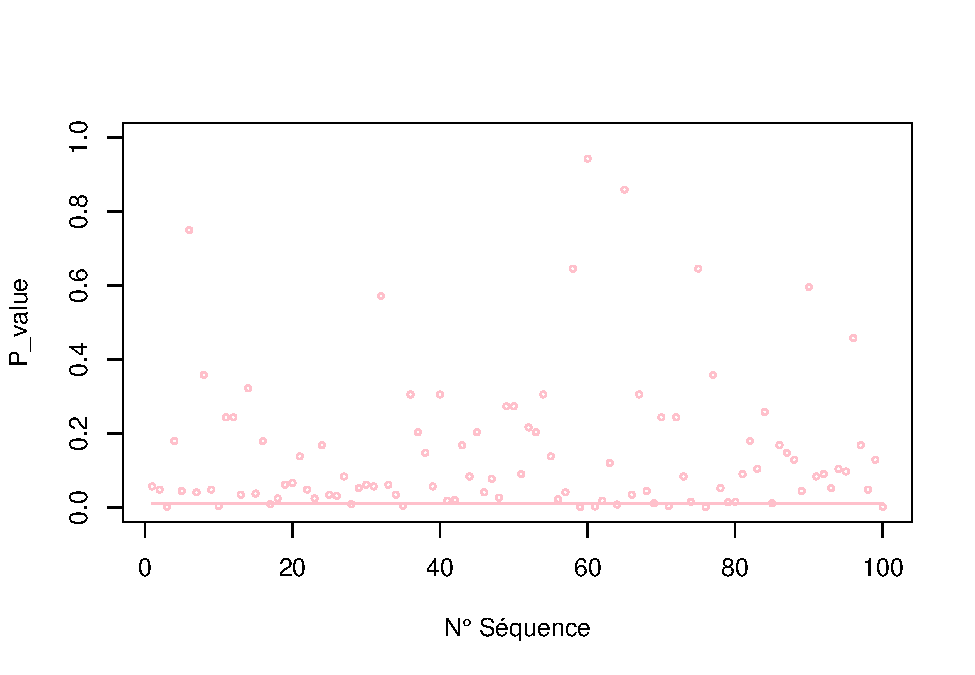
\includegraphics[width=0.5\linewidth]{CRTP_PROBA_files/figure-latex/unnamed-chunk-7-4} }\caption{Etude de la répartition des bits sur 100 séquences de cardinal 100, Graines aléatoires}\label{fig:unnamed-chunk-7}
\end{figure}
\clearpage
\subsection*{B. Tests d'ordre\footnote{Voir \textit{Runs} p. \pageref{runs}}}
\begin{figure}
\subfloat[Mersenne Twister\label{fig:unnamed-chunk-8-1}]{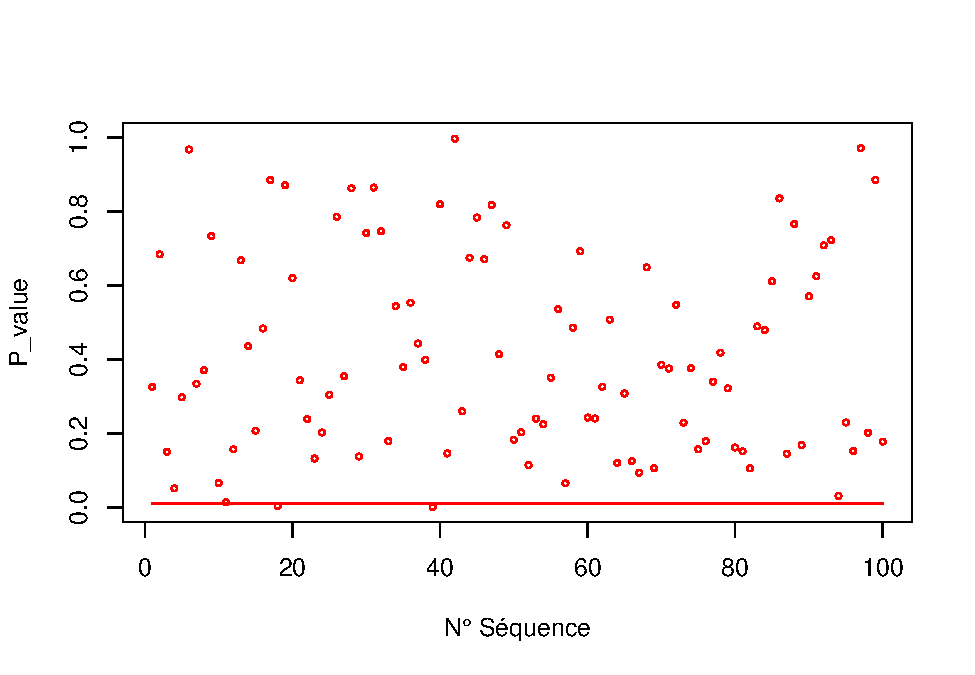
\includegraphics[width=0.5\linewidth]{CRTP_PROBA_files/figure-latex/unnamed-chunk-8-1} }\subfloat[Von Neuman\label{fig:unnamed-chunk-8-2}]{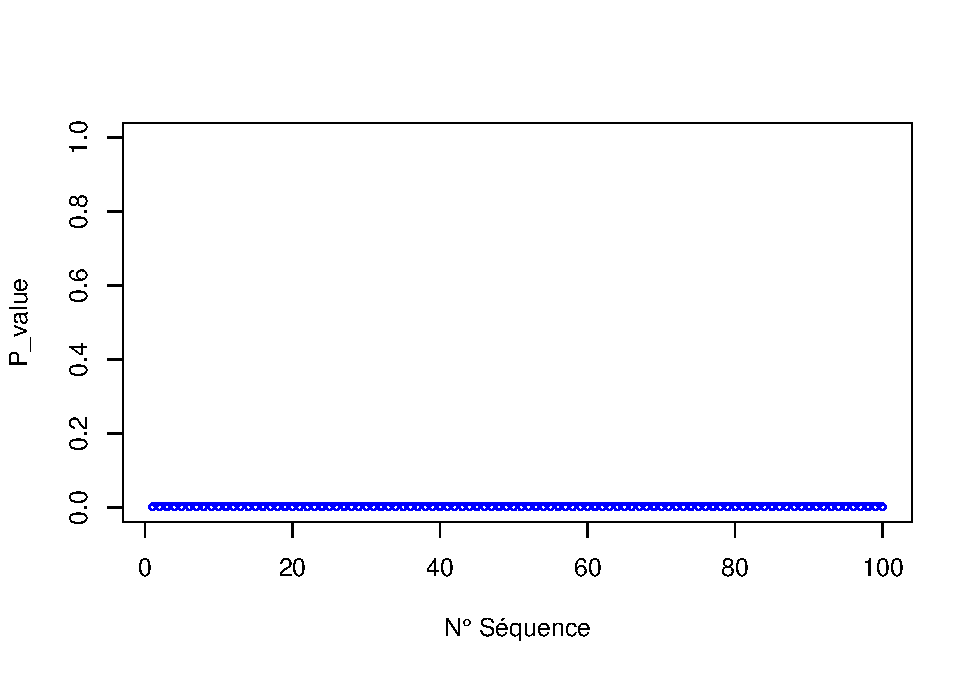
\includegraphics[width=0.5\linewidth]{CRTP_PROBA_files/figure-latex/unnamed-chunk-8-2} }\newline\subfloat[RANDU\label{fig:unnamed-chunk-8-3}]{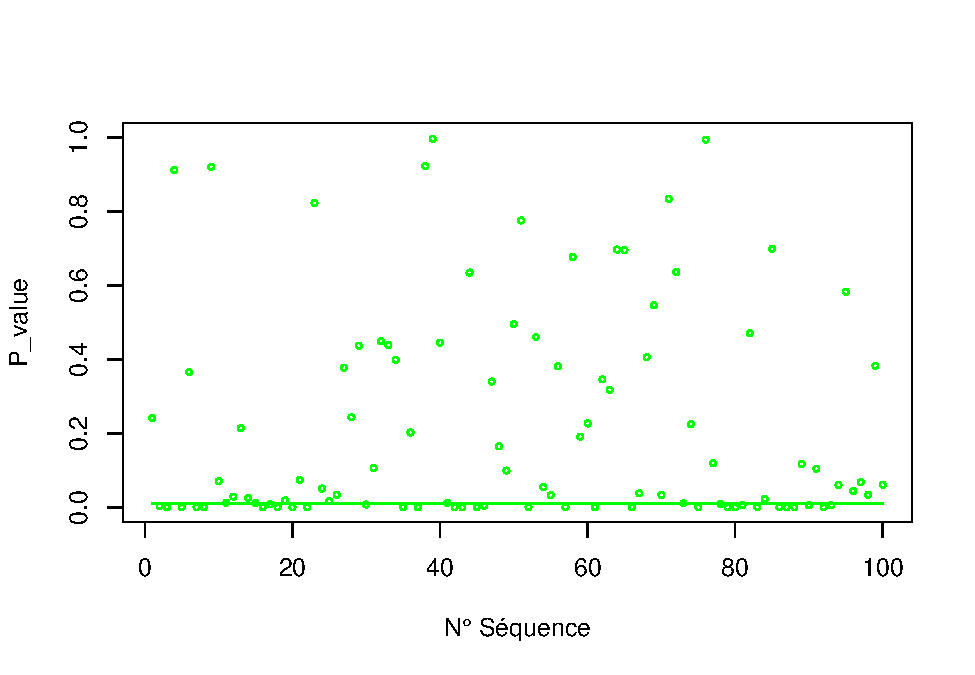
\includegraphics[width=0.5\linewidth]{CRTP_PROBA_files/figure-latex/unnamed-chunk-8-3} }\subfloat[Standard Minimal\label{fig:unnamed-chunk-8-4}]{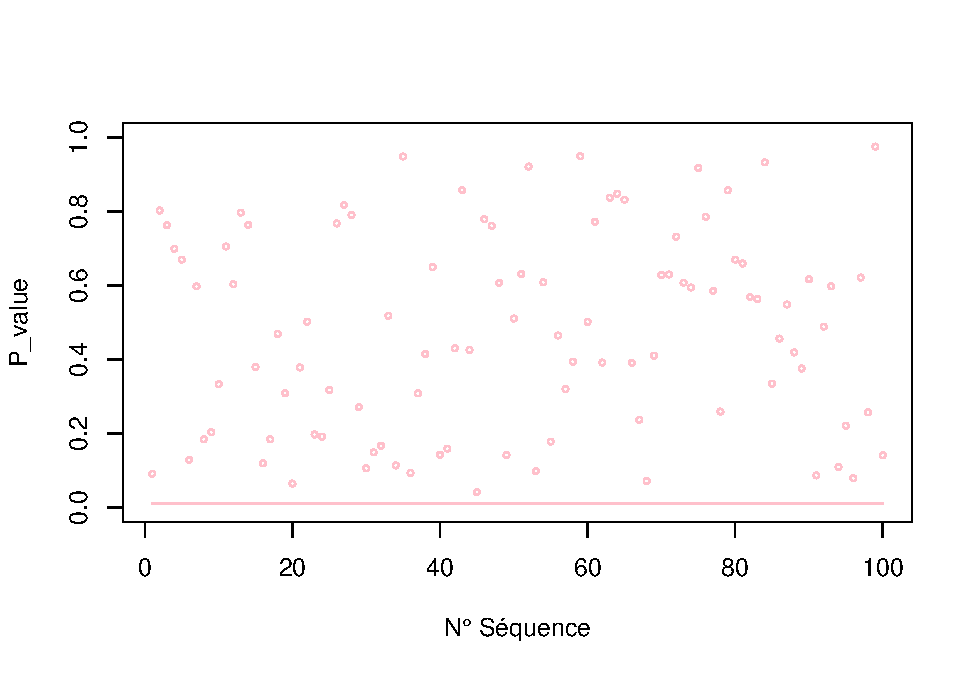
\includegraphics[width=0.5\linewidth]{CRTP_PROBA_files/figure-latex/unnamed-chunk-8-4} }\caption{Etude de l'ordonnancement des bits sur 100 séquences de cardinal 100, Graines aléatoires}\label{fig:unnamed-chunk-8}
\end{figure}
\clearpage
\subsection*{C. Tests uniformes\footnote{Voir la documentation de order.test : www.rdocumentation.org/packages/randtoolbox/versions/2.0.3/topics/order.test}}

Ici nous nous intéressons aux nombres dans leur représentation décimale
et vérifions si la séquence produite suit la loi uniforme (chaque nombre
à autant de chance d'apparaître qu'un autre).

\begin{figure}
\subfloat[Mersenne Twister\label{fig:unnamed-chunk-9-1}]{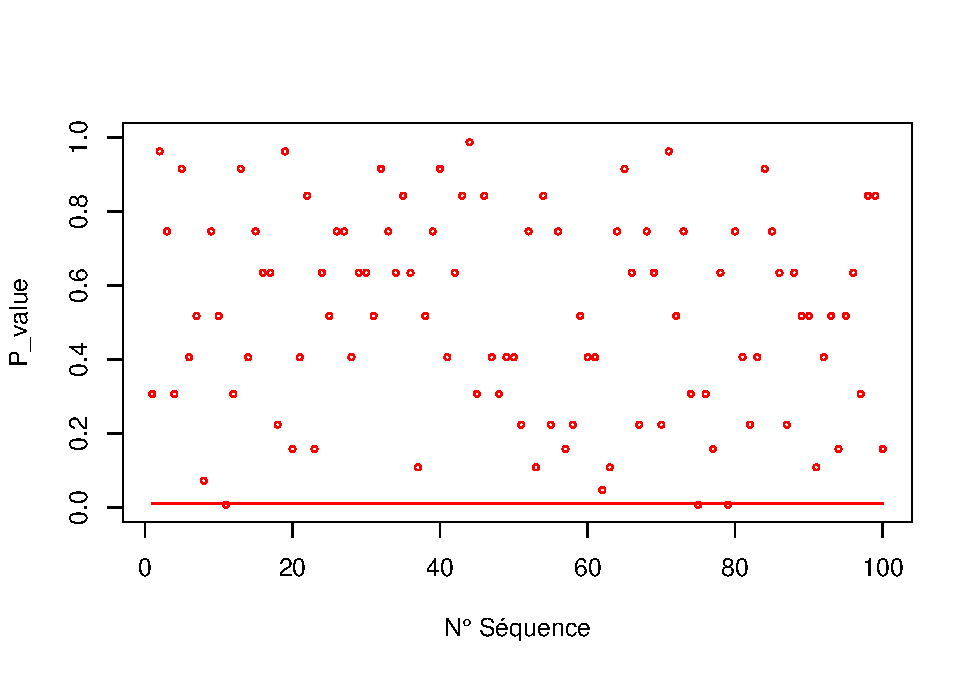
\includegraphics[width=0.5\linewidth]{CRTP_PROBA_files/figure-latex/unnamed-chunk-9-1} }\subfloat[Von Neuman\label{fig:unnamed-chunk-9-2}]{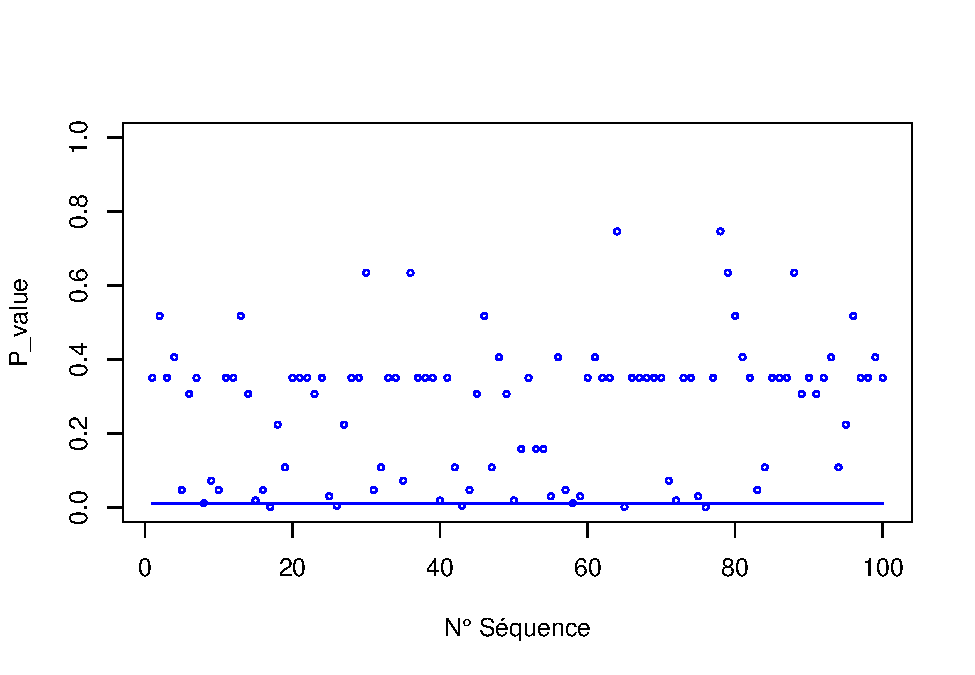
\includegraphics[width=0.5\linewidth]{CRTP_PROBA_files/figure-latex/unnamed-chunk-9-2} }\newline\subfloat[RANDU\label{fig:unnamed-chunk-9-3}]{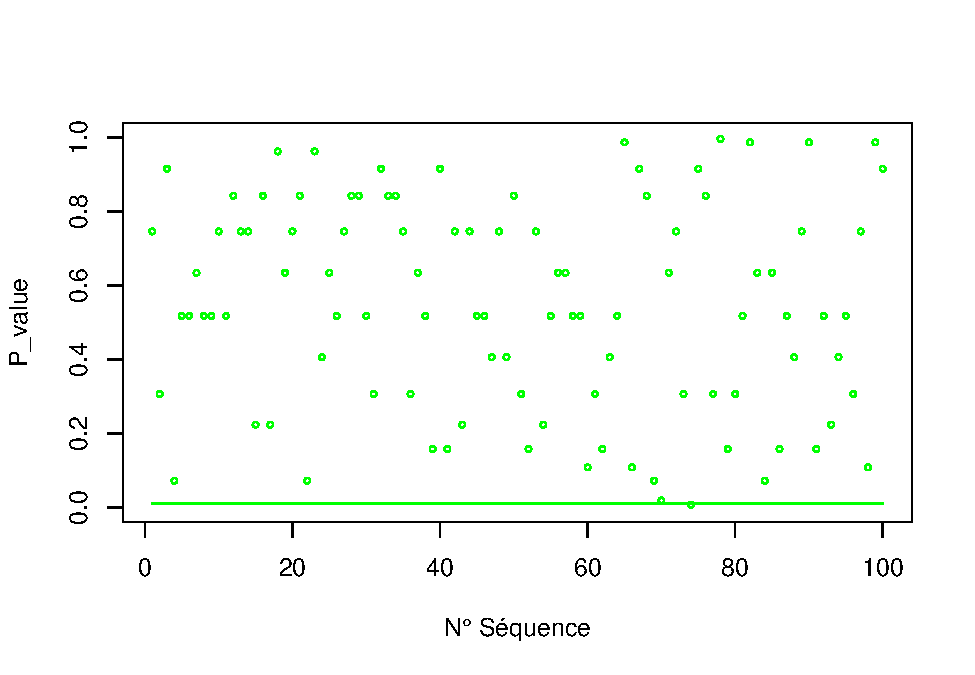
\includegraphics[width=0.5\linewidth]{CRTP_PROBA_files/figure-latex/unnamed-chunk-9-3} }\subfloat[Standard Minimal\label{fig:unnamed-chunk-9-4}]{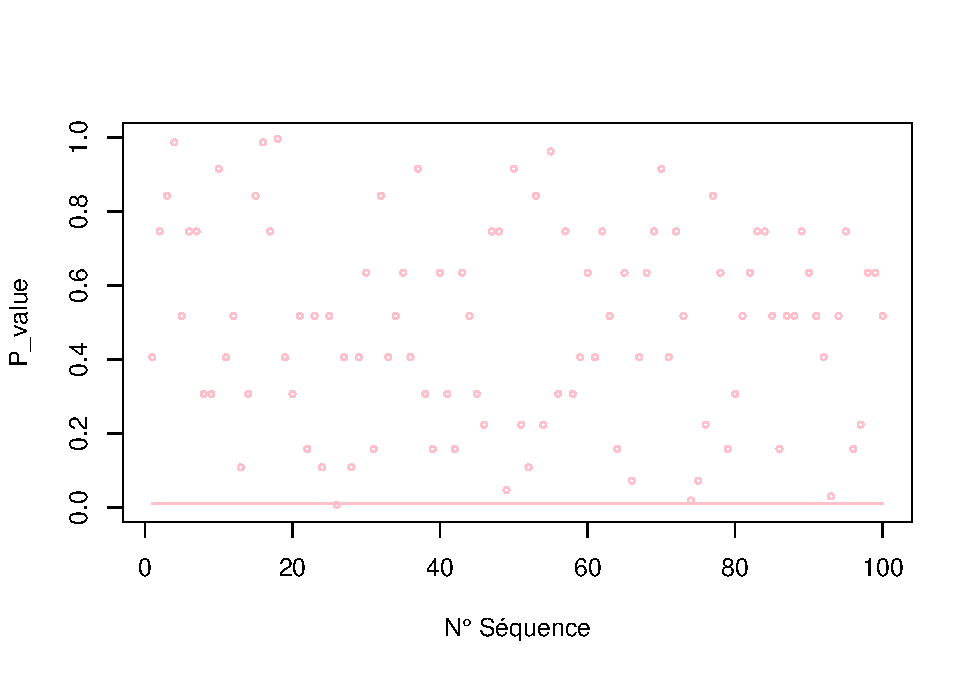
\includegraphics[width=0.5\linewidth]{CRTP_PROBA_files/figure-latex/unnamed-chunk-9-4} }\caption{Etude de la loi uniforme sur 100 séquences de cardinal 100, Graines aléatoires}\label{fig:unnamed-chunk-9}
\end{figure}

\clearpage

\part*{Partie II : Etudes des files d'attentes}
\addcontentsline{toc}{part}{Etudes des files d'attentes}

\section*{1.La file M/M/1 }
\addcontentsline{toc}{subsection}{La file M/M/1}

\paragraph{}

Nous allons visualiser l'évolution d'un système pendant une durée de 12
heures:

\begin{figure}
\subfloat[10 clients qui arrivent et 20 qui partent en moyenne par heure\label{fig:unnamed-chunk-10-1}]{\includegraphics[width=0.5\linewidth]{CRTP_PROBA_files/figure-latex/unnamed-chunk-10-1} }\subfloat[14 clients qui arrivent et 20 qui partent en moyenne par heure\label{fig:unnamed-chunk-10-2}]{\includegraphics[width=0.5\linewidth]{CRTP_PROBA_files/figure-latex/unnamed-chunk-10-2} }\newline\subfloat[20 clients qui arrivent et 20 qui partent en moyenne par heure\label{fig:unnamed-chunk-10-3}]{\includegraphics[width=0.5\linewidth]{CRTP_PROBA_files/figure-latex/unnamed-chunk-10-3} }\subfloat[30 clients qui arrivent et 20 qui partent en moyenne par heure\label{fig:unnamed-chunk-10-4}]{\includegraphics[width=0.5\linewidth]{CRTP_PROBA_files/figure-latex/unnamed-chunk-10-4} }\caption{évolution du nombre de clients dans le système pendant 12 heures de fonctionnement}\label{fig:unnamed-chunk-10}
\end{figure}

\paragraph{}

Etudions le rapport de notre file au modèle théorique.

Formule de little \#écrire formule

\begin{verbatim}
## [1] "E(N)/E(W)= 0.188382800236516"
\end{verbatim}

\begin{verbatim}
## [1] "lambda= 0.166666666666667"
\end{verbatim}

\begin{verbatim}
## [1] "E(N)/E(W)= 0.278909960801243"
\end{verbatim}

\begin{verbatim}
## [1] "lambda= 0.233333333333333"
\end{verbatim}

\begin{verbatim}
## [1] "E(N)/E(W)= 0.290244679066078"
\end{verbatim}

\begin{verbatim}
## [1] "lambda= 0.333333333333333"
\end{verbatim}

\begin{verbatim}
## [1] "E(N)/E(W)= 0.364795324718151"
\end{verbatim}

\begin{verbatim}
## [1] "lambda= 0.5"
\end{verbatim}

Nous allons maintenant vérifier \#écrire formules

\begin{verbatim}
## [1] "E(W)-E(Wa)= 2.95266325418264"
\end{verbatim}

\begin{verbatim}
## [1] "E(W)-E(Wa)= 2.45577655634133"
\end{verbatim}

\begin{verbatim}
## [1] "E(W)-E(Wa)= 3.26178478428427"
\end{verbatim}

\begin{verbatim}
## [1] "E(W)-E(Wa)= 2.77888544302346"
\end{verbatim}

\begin{verbatim}
## [1] "1/mu= 3"
\end{verbatim}

Nous allons maintenant vérifier \#écrire formules

\begin{verbatim}
## [1] "E(Na)/E(Wa) = 0.236889010414935"
\end{verbatim}

\begin{verbatim}
## [1] "lambda = 0.166666666666667"
\end{verbatim}

\begin{verbatim}
## [1] "E(W)-E(Wa) = 0.350261601553225"
\end{verbatim}

\begin{verbatim}
## [1] "lambda = 0.233333333333333"
\end{verbatim}

\begin{verbatim}
## [1] "E(W)-E(Wa) = 0.288268009374079"
\end{verbatim}

\begin{verbatim}
## [1] "lambda = 0.333333333333333"
\end{verbatim}

\begin{verbatim}
## [1] "E(W)-E(Wa) = 0.364053303633305"
\end{verbatim}

\begin{verbatim}
## [1] "lambda = 0.5"
\end{verbatim}

\section*{2.La file M/M/2 }
\addcontentsline{toc}{subsection}{La file M/M/2}

\paragraph{}

Nous allons visualiser l'évolution d'un système pendant une durée de 12
heures:

\begin{figure}
\subfloat[10 clients qui arrivent et 20 qui partent en moyenne par heure\label{fig:unnamed-chunk-14-1}]{\includegraphics[width=0.5\linewidth]{CRTP_PROBA_files/figure-latex/unnamed-chunk-14-1} }\subfloat[14 clients qui arrivent et 20 qui partent en moyenne par heure\label{fig:unnamed-chunk-14-2}]{\includegraphics[width=0.5\linewidth]{CRTP_PROBA_files/figure-latex/unnamed-chunk-14-2} }\newline\subfloat[20 clients qui arrivent et 20 qui partent en moyenne par heure\label{fig:unnamed-chunk-14-3}]{\includegraphics[width=0.5\linewidth]{CRTP_PROBA_files/figure-latex/unnamed-chunk-14-3} }\subfloat[30 clients qui arrivent et 20 qui partent en moyenne par heure\label{fig:unnamed-chunk-14-4}]{\includegraphics[width=0.5\linewidth]{CRTP_PROBA_files/figure-latex/unnamed-chunk-14-4} }\caption{évolution du nombre de clients dans le système pendant 12 heures de fonctionnement}\label{fig:unnamed-chunk-14}
\end{figure}
\part{Annexes}
\label{part:annexes}

\section*{Algorithme des générateurs}
\addcontentsline{toc}{subsection}{Algorithmes des générateurs}

\textbf{Von Neuman}

\begin{Shaded}
\begin{Highlighting}[]
\NormalTok{VonNeumann }\OtherTok{\textless{}{-}} \ControlFlowTok{function}\NormalTok{(n, }\AttributeTok{p=}\DecValTok{1}\NormalTok{, graine)}
\NormalTok{\{}
\NormalTok{  x }\OtherTok{\textless{}{-}}  \FunctionTok{rep}\NormalTok{(graine,n}\SpecialCharTok{*}\NormalTok{p}\SpecialCharTok{+}\DecValTok{1}\NormalTok{)}
  \ControlFlowTok{for}\NormalTok{(i }\ControlFlowTok{in} \DecValTok{2}\SpecialCharTok{:}\NormalTok{(n}\SpecialCharTok{*}\NormalTok{p}\SpecialCharTok{+}\DecValTok{1}\NormalTok{))}
\NormalTok{  \{}
\NormalTok{    numbers }\OtherTok{\textless{}{-}} \FunctionTok{strsplit}\NormalTok{(}\FunctionTok{format}\NormalTok{(x[i}\DecValTok{{-}1}\NormalTok{]}\SpecialCharTok{\^{}}\DecValTok{2}\NormalTok{,}\AttributeTok{scientific=}\ConstantTok{FALSE}\NormalTok{),}\StringTok{\textquotesingle{}\textquotesingle{}}\NormalTok{)[[}\DecValTok{1}\NormalTok{]]}
    \ControlFlowTok{while}\NormalTok{(}\FunctionTok{length}\NormalTok{(numbers)}\SpecialCharTok{\textgreater{}}\DecValTok{4}\NormalTok{)\{ }
\NormalTok{        numbers }\OtherTok{\textless{}{-}}\NormalTok{ numbers[}\DecValTok{2}\SpecialCharTok{:}\NormalTok{(}\FunctionTok{length}\NormalTok{(numbers)}\SpecialCharTok{{-}}\DecValTok{1}\NormalTok{)] }
\NormalTok{    \}}
\NormalTok{    x[i] }\OtherTok{\textless{}{-}} \FunctionTok{as.numeric}\NormalTok{(numbers)}\SpecialCharTok{\%*\%}\NormalTok{(}\DecValTok{10}\SpecialCharTok{\^{}}\FunctionTok{seq}\NormalTok{(}\FunctionTok{length}\NormalTok{(numbers)}\SpecialCharTok{{-}}\DecValTok{1}\NormalTok{,}\DecValTok{0}\NormalTok{,}\SpecialCharTok{{-}}\DecValTok{1}\NormalTok{))}
\NormalTok{  \}}
\NormalTok{  x }\OtherTok{\textless{}{-}} \FunctionTok{matrix}\NormalTok{(x[}\DecValTok{2}\SpecialCharTok{:}\NormalTok{(n}\SpecialCharTok{*}\NormalTok{p}\SpecialCharTok{+}\DecValTok{1}\NormalTok{)],}\AttributeTok{nrow=}\NormalTok{n,}\AttributeTok{ncol=}\NormalTok{p)}
  \FunctionTok{return}\NormalTok{(x)}
\NormalTok{\}}
\end{Highlighting}
\end{Shaded}

\textbf{Mersenne Twister}

\begin{Shaded}
\begin{Highlighting}[]
\NormalTok{MersenneTwister }\OtherTok{\textless{}{-}} \ControlFlowTok{function}\NormalTok{(n, }\AttributeTok{p=}\DecValTok{1}\NormalTok{, graine)}
\NormalTok{\{}
  \FunctionTok{set.seed}\NormalTok{(graine,}\AttributeTok{kind=}\StringTok{\textquotesingle{}Mersenne{-}Twister\textquotesingle{}}\NormalTok{)}
\NormalTok{  x }\OtherTok{\textless{}{-}} \FunctionTok{sample.int}\NormalTok{(}\DecValTok{2}\SpecialCharTok{\^{}}\DecValTok{32{-}1}\NormalTok{,n}\SpecialCharTok{*}\NormalTok{p)}
\NormalTok{  x }\OtherTok{\textless{}{-}} \FunctionTok{matrix}\NormalTok{(x,}\AttributeTok{nrow=}\NormalTok{n,}\AttributeTok{ncol=}\NormalTok{p)}
  \FunctionTok{return}\NormalTok{(x)}
\NormalTok{\}}
\end{Highlighting}
\end{Shaded}

\textbf{RANDU}

\begin{Shaded}
\begin{Highlighting}[]
\NormalTok{RANDU }\OtherTok{\textless{}{-}} \ControlFlowTok{function}\NormalTok{(}\AttributeTok{n=}\DecValTok{1}\NormalTok{,}\AttributeTok{k =} \DecValTok{10}\NormalTok{,graine)}
\NormalTok{\{}
\NormalTok{  x }\OtherTok{\textless{}{-}}  \FunctionTok{rep}\NormalTok{(graine,k}\SpecialCharTok{*}\NormalTok{n}\SpecialCharTok{+}\DecValTok{1}\NormalTok{)}
  \ControlFlowTok{for}\NormalTok{ (i }\ControlFlowTok{in} \DecValTok{2}\SpecialCharTok{:}\NormalTok{(k}\SpecialCharTok{*}\NormalTok{n}\SpecialCharTok{+}\DecValTok{1}\NormalTok{)) \{}
\NormalTok{    x[i] }\OtherTok{\textless{}{-}}\NormalTok{ (}\DecValTok{65539}\SpecialCharTok{*}\NormalTok{x[i}\DecValTok{{-}1}\NormalTok{])}\SpecialCharTok{\%\%}\NormalTok{(}\DecValTok{2}\SpecialCharTok{\^{}}\DecValTok{31}\NormalTok{)}
\NormalTok{  \}}
\NormalTok{  x }\OtherTok{\textless{}{-}} \FunctionTok{matrix}\NormalTok{(x[}\DecValTok{2}\SpecialCharTok{:}\NormalTok{(k}\SpecialCharTok{*}\NormalTok{n}\SpecialCharTok{+}\DecValTok{1}\NormalTok{)],}\AttributeTok{nrow=}\NormalTok{n,}\AttributeTok{ncol=}\NormalTok{k)}
  
  \FunctionTok{return}\NormalTok{(x)}
\NormalTok{\}}
\end{Highlighting}
\end{Shaded}

\textbf{Standard Minimal}

\begin{Shaded}
\begin{Highlighting}[]
\NormalTok{StandardMinimal }\OtherTok{\textless{}{-}} \ControlFlowTok{function}\NormalTok{(}\AttributeTok{n=}\DecValTok{1}\NormalTok{,}\AttributeTok{k =} \DecValTok{10}\NormalTok{,graine)}
\NormalTok{\{}
\NormalTok{  x }\OtherTok{\textless{}{-}}  \FunctionTok{rep}\NormalTok{(graine,k}\SpecialCharTok{*}\NormalTok{n}\SpecialCharTok{+}\DecValTok{1}\NormalTok{)}
  
  \ControlFlowTok{for}\NormalTok{ (i }\ControlFlowTok{in} \DecValTok{2}\SpecialCharTok{:}\NormalTok{(k}\SpecialCharTok{*}\NormalTok{n}\SpecialCharTok{+}\DecValTok{1}\NormalTok{)) \{}
\NormalTok{    x[i] }\OtherTok{\textless{}{-}}\NormalTok{ (}\DecValTok{16807}\SpecialCharTok{*}\NormalTok{x[i}\DecValTok{{-}1}\NormalTok{])}\SpecialCharTok{\%\%}\NormalTok{ (}\DecValTok{2}\SpecialCharTok{\^{}}\DecValTok{31{-}1}\NormalTok{)}
\NormalTok{  \}}
  
\NormalTok{  x }\OtherTok{\textless{}{-}} \FunctionTok{matrix}\NormalTok{(x[}\DecValTok{2}\SpecialCharTok{:}\NormalTok{(k}\SpecialCharTok{*}\NormalTok{n}\SpecialCharTok{+}\DecValTok{1}\NormalTok{)],}\AttributeTok{nrow=}\NormalTok{n,}\AttributeTok{ncol=}\NormalTok{k)}
  
  \FunctionTok{return}\NormalTok{(x)}
\NormalTok{\}}
\end{Highlighting}
\end{Shaded}

\section*{Binary}
\addcontentsline{toc}{subsection}{Algorithme de \textit{binary}}

\label{subsec:binary}

\begin{Shaded}
\begin{Highlighting}[]
\NormalTok{binary }\OtherTok{\textless{}{-}} \ControlFlowTok{function}\NormalTok{(x)}
\NormalTok{\{}
  \ControlFlowTok{if}\NormalTok{((x}\SpecialCharTok{\textless{}}\DecValTok{2}\SpecialCharTok{\^{}}\DecValTok{31}\NormalTok{)}\SpecialCharTok{\&}\NormalTok{(x}\SpecialCharTok{\textgreater{}=}\DecValTok{0}\NormalTok{))}
    \FunctionTok{return}\NormalTok{( }\FunctionTok{as.integer}\NormalTok{(}\FunctionTok{intToBits}\NormalTok{(}\FunctionTok{as.integer}\NormalTok{(x))) )}
  \ControlFlowTok{else}\NormalTok{\{}
    \ControlFlowTok{if}\NormalTok{((x}\SpecialCharTok{\textless{}}\DecValTok{2}\SpecialCharTok{\^{}}\DecValTok{32}\NormalTok{)}\SpecialCharTok{\&}\NormalTok{(x}\SpecialCharTok{\textgreater{}}\DecValTok{0}\NormalTok{))}
      \FunctionTok{return}\NormalTok{( }\FunctionTok{c}\NormalTok{(}\FunctionTok{binary}\NormalTok{(x}\DecValTok{{-}2}\SpecialCharTok{\^{}}\DecValTok{31}\NormalTok{)[}\DecValTok{1}\SpecialCharTok{:}\DecValTok{31}\NormalTok{], }\DecValTok{1}\NormalTok{) )}
    \ControlFlowTok{else}\NormalTok{\{}
      \FunctionTok{cat}\NormalTok{(}\StringTok{\textquotesingle{}Erreur dans binary : le nombre etudie n est pas un entier positif en 32 bits.}\SpecialCharTok{\textbackslash{}n}\StringTok{\textquotesingle{}}\NormalTok{)}
      \FunctionTok{return}\NormalTok{(}\FunctionTok{c}\NormalTok{())}
\NormalTok{    \}}
\NormalTok{  \}}
\NormalTok{\}}
\end{Highlighting}
\end{Shaded}

\section*{Graines}

\begin{verbatim}
##   [1] 1.3e+09 1.0e+09 1.4e+09 1.7e+09 7.7e+08 1.3e+09 3.9e+08 7.2e+08 1.2e+09
##  [10] 7.1e+08 1.5e+09 1.5e+08 1.5e+09 2.2e+08 1.6e+09 2.4e+07 1.9e+08 2.8e+08
##  [19] 1.0e+09 1.8e+09 1.1e+08 6.5e+08 4.0e+08 1.8e+09 2.0e+09 1.5e+09 2.6e+08
##  [28] 1.4e+09 7.3e+08 9.3e+08 1.2e+09 3.7e+08 1.4e+09 2.0e+09 8.1e+08 2.1e+09
##  [37] 9.3e+08 4.6e+08 1.2e+09 2.0e+09 2.0e+09 1.1e+09 5.6e+08 2.0e+09 1.7e+09
##  [46] 2.1e+09 8.2e+08 1.4e+09 2.1e+09 2.0e+09 3.9e+08 5.3e+08 1.6e+08 8.5e+08
##  [55] 2.1e+09 2.1e+09 7.7e+08 1.1e+09 1.9e+09 2.0e+09 9.0e+08 2.1e+08 1.2e+09
##  [64] 1.7e+09 2.0e+09 1.6e+09 1.3e+09 1.8e+09 1.5e+09 1.9e+09 7.2e+08 1.8e+09
##  [73] 1.8e+09 1.5e+09 1.5e+08 1.3e+09 1.4e+09 1.6e+09 1.6e+09 5.1e+08 8.7e+07
##  [82] 1.8e+09 6.4e+08 1.2e+09 1.8e+09 1.1e+08 1.8e+09 1.1e+09 2.1e+09 1.5e+09
##  [91] 1.4e+09 3.7e+08 9.4e+08 5.3e+07 1.9e+09 4.3e+08 5.4e+08 2.1e+09 1.5e+09
## [100] 1.8e+09
\end{verbatim}

\section*{Algorithmes des tests}
\addcontentsline{toc}{subsection}{Algorithmes des tests}

\textbf{Frequency ou l'étude de la répartition binaire}
\label{frequency}

\begin{Shaded}
\begin{Highlighting}[]
\NormalTok{Frequency }\OtherTok{\textless{}{-}} \ControlFlowTok{function}\NormalTok{(x, nb)}
\NormalTok{\{}
\NormalTok{  cn }\OtherTok{\textless{}{-}} \FunctionTok{binary}\NormalTok{(x[}\DecValTok{1}\NormalTok{])}
\NormalTok{  b }\OtherTok{\textless{}{-}}\NormalTok{ cn[}\DecValTok{1}\SpecialCharTok{:}\NormalTok{nb]}
  \ControlFlowTok{for}\NormalTok{(i }\ControlFlowTok{in} \DecValTok{2}\SpecialCharTok{:}\FunctionTok{length}\NormalTok{(x))\{}
\NormalTok{    cn }\OtherTok{\textless{}{-}} \FunctionTok{binary}\NormalTok{(x[i])}
\NormalTok{    b }\OtherTok{\textless{}{-}} \FunctionTok{c}\NormalTok{(b,cn[}\DecValTok{1}\SpecialCharTok{:}\NormalTok{nb])}
\NormalTok{  \}}
  \ControlFlowTok{for}\NormalTok{(i }\ControlFlowTok{in} \DecValTok{1}\SpecialCharTok{:}\FunctionTok{length}\NormalTok{(b))\{}
    \ControlFlowTok{if}\NormalTok{(b[i]}\SpecialCharTok{==}\DecValTok{0}\NormalTok{)}
\NormalTok{      b[i] }\OtherTok{\textless{}{-}} \SpecialCharTok{{-}}\DecValTok{1}
\NormalTok{  \}}
  
\NormalTok{  S }\OtherTok{\textless{}{-}} \FunctionTok{sum}\NormalTok{(b)}
  
\NormalTok{  sObs }\OtherTok{\textless{}{-}} \FunctionTok{abs}\NormalTok{(S)}\SpecialCharTok{/}\FunctionTok{sqrt}\NormalTok{(}\FunctionTok{length}\NormalTok{(b))}
  
\NormalTok{  p }\OtherTok{\textless{}{-}} \DecValTok{2}\SpecialCharTok{*}\NormalTok{(}\DecValTok{1}\SpecialCharTok{{-}}\FunctionTok{pnorm}\NormalTok{(sObs,}\DecValTok{0}\NormalTok{,}\DecValTok{1}\NormalTok{))}
  
  \FunctionTok{return}\NormalTok{(p)}
\NormalTok{\}}
\end{Highlighting}
\end{Shaded}

\textbf{Runs ou l'étude de l'ordre binaire} \label{runs}

\begin{Shaded}
\begin{Highlighting}[]
\NormalTok{Runs }\OtherTok{\textless{}{-}} \ControlFlowTok{function}\NormalTok{(x, nb)}
\NormalTok{\{}
\NormalTok{  cn }\OtherTok{\textless{}{-}} \FunctionTok{binary}\NormalTok{(x[}\DecValTok{1}\NormalTok{])}
\NormalTok{  b }\OtherTok{\textless{}{-}}\NormalTok{ cn[}\DecValTok{1}\SpecialCharTok{:}\NormalTok{nb]}
  \ControlFlowTok{for}\NormalTok{(i }\ControlFlowTok{in} \DecValTok{2}\SpecialCharTok{:}\FunctionTok{length}\NormalTok{(x))\{}
\NormalTok{    cn }\OtherTok{\textless{}{-}} \FunctionTok{binary}\NormalTok{(x[i])}
\NormalTok{    b }\OtherTok{\textless{}{-}} \FunctionTok{c}\NormalTok{(b,cn[}\DecValTok{1}\SpecialCharTok{:}\NormalTok{nb])}
\NormalTok{  \}}
  \CommentTok{\#Pre{-}test}
\NormalTok{  S }\OtherTok{\textless{}{-}} \FunctionTok{sum}\NormalTok{(b)}
\NormalTok{  pi }\OtherTok{\textless{}{-}}\NormalTok{ S}\SpecialCharTok{/}\FunctionTok{length}\NormalTok{(b)}
  
  \ControlFlowTok{if}\NormalTok{(}\FunctionTok{abs}\NormalTok{(pi}\SpecialCharTok{{-}}\NormalTok{(}\DecValTok{1}\SpecialCharTok{/}\DecValTok{2}\NormalTok{))}\SpecialCharTok{\textgreater{}=}\NormalTok{(}\DecValTok{2}\SpecialCharTok{/}\FunctionTok{sqrt}\NormalTok{(}\FunctionTok{length}\NormalTok{(b))))\{}
    \FunctionTok{return}\NormalTok{(}\FloatTok{0.0}\NormalTok{)}
\NormalTok{  \}}
  
  \CommentTok{\#Test}
\NormalTok{  VnObs }\OtherTok{\textless{}{-}} \DecValTok{0}
  \ControlFlowTok{for}\NormalTok{(i }\ControlFlowTok{in} \DecValTok{1}\SpecialCharTok{:}\NormalTok{(}\FunctionTok{length}\NormalTok{(b)}\SpecialCharTok{{-}}\DecValTok{1}\NormalTok{))\{}
    \ControlFlowTok{if}\NormalTok{(b[i}\SpecialCharTok{+}\DecValTok{1}\NormalTok{]}\SpecialCharTok{!=}\NormalTok{b[i])}
\NormalTok{      VnObs }\OtherTok{\textless{}{-}}\NormalTok{ VnObs }\SpecialCharTok{+} \DecValTok{1}
\NormalTok{  \}}
\NormalTok{  VnObs }\OtherTok{\textless{}{-}}\NormalTok{ VnObs }\SpecialCharTok{+} \DecValTok{1}
\NormalTok{  frac }\OtherTok{\textless{}{-}}\NormalTok{ (}\FunctionTok{abs}\NormalTok{(VnObs}\DecValTok{{-}2}\SpecialCharTok{*}\FunctionTok{length}\NormalTok{(b)}\SpecialCharTok{*}\NormalTok{pi}\SpecialCharTok{*}\NormalTok{(}\DecValTok{1}\SpecialCharTok{{-}}\NormalTok{pi))}\SpecialCharTok{/}\NormalTok{(}\DecValTok{2}\SpecialCharTok{*}\FunctionTok{sqrt}\NormalTok{(}\FunctionTok{length}\NormalTok{(b))}\SpecialCharTok{*}\NormalTok{pi}\SpecialCharTok{*}\NormalTok{(}\DecValTok{1}\SpecialCharTok{{-}}\NormalTok{pi)))}
\NormalTok{  P }\OtherTok{\textless{}{-}} \DecValTok{2}\SpecialCharTok{*}\NormalTok{(}\DecValTok{1}\SpecialCharTok{{-}}\FunctionTok{pnorm}\NormalTok{(frac,}\DecValTok{0}\NormalTok{,}\DecValTok{1}\NormalTok{))}
  
  \FunctionTok{return}\NormalTok{(P)}
\NormalTok{\}}
\end{Highlighting}
\end{Shaded}


\end{document}
